\section{Report Generation}

Generating Reports
\newline
If you should so wish it is possible to generate an XML version of the current state the application is in. This report will show you an overview of all your projects, teams, skills, people, team allocations etc so that you can get a general feel for everything in the current state.
\newline\newline
In order to generate this report all you need to do is click on File/Generate Report. When you do a dialog will appear asking where you would like to save the report and what file format you want to save it as (this defaults to XML, but if you want you can save it as a .report file). Once you have selected a location and pressed save then if you go to the location that you saved the report in and open the file you will have an XML representation of the file as shown in the diagram below.

\begin{figure}[H]
\centering
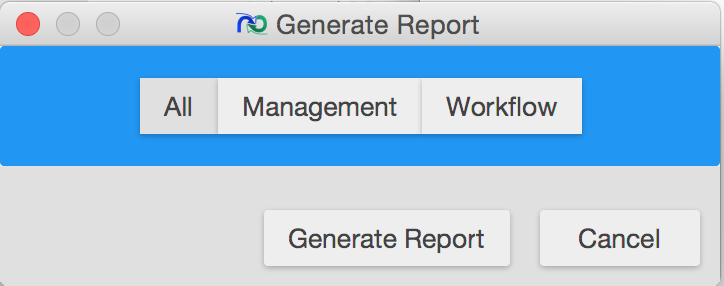
\includegraphics[width=\textwidth]{images/screenshots/report1.PNG}
\caption{The Display Choice Picker}
\label{fig:new_project}
\end{figure}